\documentclass{article}

\usepackage[left=2cm,right=2cm, top=2cm, bottom = 2cm]{geometry}
\usepackage{amsfonts}

\usepackage{amsmath}
\usepackage{xcolor}

\usepackage{tikz}
\usepackage{subfigure}



\pagestyle{empty}

\setlength{\tabcolsep}{15pt}

\newcommand{\ihat}{\hat\i}
\newcommand{\jhat}{\hat\j}
\newcommand{\khat}{\hat{k}}

\newcommand{\deriv}[3][]{\frac{\mathrm{d}^{#1}#2}{\mathrm{d}#3^{#1}}}
\newcommand{\diff}{\;\mathrm{d}}

\newcommand{\norm}[1]{\left|\kern-1pt\left|#1\right|\kern-1pt\right|}

\newcommand{\braket}[2]{\left\langle #1 \mid #2 \right\rangle}

\let\uline\underline



\begin{document}

\title{Scalar Products and Geometry}
\date{}

\maketitle
\thispagestyle{empty}

\Large

\textbf{\underline{Objective: To understand the scalar product of vectors in 2 and 3}}

\textbf{\underline{dimensions and use it to solve geometry problems.}}



\vspace{5mm}



\textbf{Warm-up: The Cosine Rule:}\bigskip



Recall the \textbf{cosine rule}: in a triangle as below,
\begin{center}
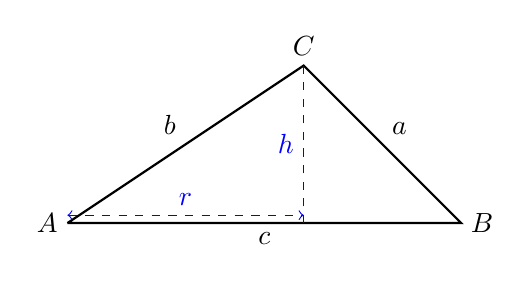
\begin{tikzpicture}
	\draw[thick] (0,0) -- (5,0) -- (3,2) -- (0,0);
	\node[left] at (0,0) {$A$};
	\node[right] at (5,0) {$B$};
	\node[above] at (3,2) {$C$};
	\node[below] at (2.5,0) {$c$};
	\node[above right] at (4,1) {$a$};
	\node[above left] at (1.5,1) {$b$};
	
	\draw[blue,dashed] (3,0) -- (3,2);
	\node[blue,left] at (3,1) {$h$};
	\draw[<->,blue,dashed] (0,0.1) -- (3,0.1);
	\node[above,blue] at (1.5,0.1) {$r$};
\end{tikzpicture}
\end{center}
\[a^2=b^2+c^2-2bc\cos(A).\]

We will prove this.\bigskip



\begin{enumerate}
	\item Use Pythagoras' Theorem to express $a^2$ in terms of $h$, $c$ and $r$. %a^2=h^2+(c-r)^2
	\item Use SohCahToa to express $h$ and $r$ in terms of $b$ and $A$. %h=b\sin(A), r=b\cos(A)
	\item Substitute your expressions from part 2 into your expression from part 1 and deduce the cosine rule. %a^2=b^2\sin^2(A) + c^2-2bc\cos(A) + b^2\cos^2(A)
\end{enumerate}




\clearpage

\textbf{The Scalar Product:}\bigskip


Let $u,v\in\mathbb{R}^2$ be two vectors in the plane:
\[u=\left(\begin{array}{c}u_1\\u_2\end{array}\right)\qquad v=\left(\begin{array}{c}v_1\\v_2\end{array}\right).\]
Define the \textbf{scalar product} or \textbf{dot product}
\[u\cdot v = u_1v_1+u_2v_2.\]

The scalar product is an example of a general notion called an inner product. For this reason you may occasionally hear it referred to as the ``euclidean inner product.'' An inner product is essentially what you need to be able to do geometry. There are three properties an inner product must satisfy; we will prove that the dot product satisfies them, and some consequences:

\begin{enumerate}
	\item Prove that the dot product is \textbf{symmetric}:
		\[u\cdot v=v\cdot u\]
		for any vectors $u$ and $v$.
	\item Prove that the dot product is \textbf{linear in the first argument}:
		\[(\lambda u+\mu v)\cdot w = \lambda(u\cdot w) + \mu(v\cdot w)\]
		for any vectors $u$, $v$, and $w$, and any scalars $\lambda$ and $\mu$.
	\item Prove that the dot product is \textbf{positive-definite}:
		\[u\cdot u\geq 0\]
		for any vector $u$, and if $u\cdot u=0$, then $u=\uline{0}$.
	\item Using only the three properties you have just shown, prove also that the dot product is linear in the \textit{second} argument:
		\[u\cdot(\lambda v+\mu w) = \lambda(u\cdot v) + \mu(u\cdot w)\]
		for any scalars $\lambda$ and $\mu$ and vectors $u$, $v$, and $w$. Because the dot product is linear in both the first and second argument, we say it is \textbf{bilinear}.
	\item Using the properties you have proved, show that
		\[v\cdot \uline{0}=\uline{0}\]
		for any vector $v$.
\end{enumerate}




\clearpage








\textbf{Theory---Scalar Products and Angles:}\bigskip


We defined the dot product of two vectors in terms of their components: we multiply each component of $u$ by the corresponding component of $v$ and add them up. There is another formula for the dot product:
\[u\cdot v = |u|.|v|\cos(\theta),\]
where $\theta$ is the angle between $u$ and $v$, and $|u|$, $|v|$ are the lengths of $u$ and $v$ respectively:
\[|u|=\sqrt{u_1^2+u_2^2}.\]

This formula is the key to why inner products are so important in geometry. We will now prove it.\medskip

\begin{center}
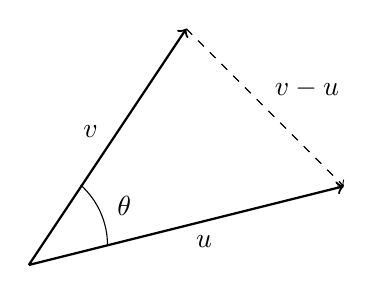
\begin{tikzpicture}
	\draw[->,thick] (0,0) -- (4,1);
	\node[below right] at (2,0.5) {$u$};
	
	\draw[->,thick] (0,0) -- (2,3);
	\node[above left] at (1,1.5) {$v$};
	
	\draw[->,dashed] (2,3) -- (4,1);
	\node[above right] at (3,2) {$v-u$};
	
	\draw (1,0.25) arc (0:48:1.031);
	\node[above right] at (1,0.5) {$\theta$};
\end{tikzpicture}
\end{center}

\begin{enumerate}
	\item First we need to relate the length of a vector to dot products. Show that, for any vector $u$:
		\[|u|=\sqrt{u\cdot u}.\]
	\item Consider the diagram above. Apply the cosine rule to express $|v-u|^2$ in terms of $|u|$, $|v|$, and $\theta$.
	\item By part 1, $|v-u|^2=(v-u)\cdot(v-u)$. Expand out the brackets (using bilinearity) and substitute into your expression from part 2 to deduce the cosine formula for $u\cdot v$.
\end{enumerate}\bigskip


So far we have worked in 2 dimensions. In 3D, we define the dot product by
\[\left(\begin{array}{c}u_1\\u_2\\u_3\end{array}\right)\cdot\left(\begin{array}{c}v_1\\v_2\\v_3\end{array}\right)=u_1v_1+u_2v_2+u_3v_3.\]

The properties of the dot product we verified in 2 dimensions still hold in 3, by essentially the same arguments. In particular, the formula relating the dot product of two vectors to their lengths and the angle between them is valid in 3D.









\clearpage




\textbf{Practice:}\bigskip

\begin{enumerate}
	\item Find the angle between the position vectors of the points $(1,3)$ and $(4,7)$.
	\item The line $L_1$ passes through the origin and the point $(-2,1)$. The line $L_2$ passes through $(-2,1)$ and $(0,4)$. Find the acute angle between $L_1$ and $L_2$.
	\item Find the angle between the vectors
		\[\left(\begin{array}{c}1\\0\end{array}\right)\quad \mbox{ and } \quad \left(\begin{array}{c}1\\-1\end{array}\right).\]
	\item Let $u$ and $v$ be non-zero vectors. Show that $u\cdot v=0$ if and only if $u$ and $v$ are perpendicular.
	\item Which pairs of the following vectors are perpendicular?
		\[u=\left(\begin{array}{c} 1\\3\\4\end{array}\right),\;v=\left(\begin{array}{c} 0\\7\\-2\end{array}\right),\;w=\left(\begin{array}{c} 0\\2\\7\end{array}\right),\;x=\left(\begin{array}{c} 13\\-7\\2\end{array}\right).\]
\end{enumerate}








\clearpage










\textbf{Lines in $\mathbb{R}^2$ and $\mathbb{R}^3$:}\bigskip

Intuitively, a line can be specified by giving a point on the line and a direction. A vector has both a direction and a length, so giving a point and a vector should specify a line if we ignore the length of the vector and just use the direction. If $p$ is the position vector of a point on the line, and $v$ is any non-zero vector in the direction given by the line, then any other point $r$ on the line can be reached from $p$ by moving some distance $\lambda$ in the direction $v$ (or the opposite direction, in which case we just take $\lambda$ to be negative). So any point $r$ on the line has the form
\[r=p+\lambda v\]
for some $\lambda\in\mathbb{R}$. Not only does every point on the line through $p$ in direction $v$ have this form, but every point of this form lies on the line; for if $r=p+\lambda v$ for some $\lambda$, then the displacement vector from $p$ to $r$ is $r-p=\lambda v$, which is in the direction of $v$, so moving from $p$ to $r$ means moving in the direction of the line.

Another way to specify a line is to give two points on it, $p$ and $q$. It is easy to convert this into the previous information of a point on the line and vector in the direction of the line: for the displacement vector $p-q$ must lie along the line, so we can write a general point $r$ on the line as
\[r=p+\lambda(p-q).\]

Give the vector equations of the lines:
\begin{enumerate}
	\item passing through the point $(3,2)$ and parallel to the vector $(4,-1)$.
	\item passing through $(-1,3)$ and $(2,0)$.
	\item in the plane with equation $y=3x+2$.
	\item in the plane with equation $x=-9$.
	\item passing through (7,0,0) and parallel to the vector $(3,1,-4)$.
	\item passing through $(1,1,1)$ and $(1,-1,1)$.
\end{enumerate}



\clearpage











\textbf{Dimensions and Linear Equations:}\bigskip


In 2D, we can specify a line by its equation, $ax+by=c$, where $a$, $b$, and $c$ are real constants. How does this generalise to 3D?

Dimension can be thought of as the number of independent pieces of information you need to give to specify a point; for instance, in 2D space, you need to give two pieces of information (an $x$-coordinate and a $y$-coordinate, in cartesians, or an $r$-coordinate and a $\theta$-coordinate in polars) to specify a point. On the other hand, in 3D space, you need to give three pieces of information (an $x$-, a $y$-, and a $z$-coordinate, for instance) to specify a point.

An equation is a piece of information; so in the plane, where you have two dimensions, giving an equation gives one of the two pieces of information you need to specify a point, so you only need one more piece of information; therefore, the solutions of that equation must form a 1D space---a line. Once you know that a point satisfies the equation $ax+by=c$, you only need one more piece of information to find that point (either one of its coordinates, or any other line it lies on!), so the solutions of that equation form a 1D subspace of the plane.

On the other hand, in 3D space, an equation still provides one piece of information, so you still need two more pieces to specify a point; so the solutions of the equation must form a 2D subspace---a plane! Giving \textit{two} equations means you only need one more, so the solutions of two simultaneous linear equations in 3D space form a 1D subspace---a line. There is a slight caveat here: the equations must be independent; for instance, $x+y+z=1$ and $2x+2x+2z=2$ are not independent, so don't count as two separate equations.\bigskip


So in 3D space a line is given by two equations in $x$, $y$, and $z$ simultaneously; neither one by itself will suffice. If the vector equation of the line is
\[\left(\begin{array}{c}x\\y\\z\end{array}\right)=\left(\begin{array}{c}p_1\\p_2\\p_3\end{array}\right)+\lambda\left(\begin{array}{c}v_1\\v_2\\v_3\end{array}\right),\]
then we can split this as three simultaneous linear equations (one for each coordinate):
\begin{align*}
	x&=p_1+\lambda v_1\\
	y&=p_2+\lambda v_2\\
	z&=p_3+\lambda v_3.
\end{align*}
We then eliminate $\lambda$ to find the cartesian equations of the line. Examples will clarify.



\clearpage




\textbf{Cartesian Equations of Lines:}\bigskip

Find the cartesian equations of the line
\[r=\left(\begin{array}{c}1\\0\\-3\end{array}\right)+\lambda \left(\begin{array}{c}2\\2\\-1\end{array}\right).\]
\vfill

Find the vector equation of the line
\[\frac{x-1}{3}=\frac{y}{2}=\frac{z-9}{5}.\]
\vfill



\begin{enumerate}
	\item Find the cartesian equations of the following lines:
		\begin{enumerate}
			\item $r=\left(\begin{array}{c}2\\-9\\5\end{array}\right)+\lambda \left(\begin{array}{c}18\\11\\1\end{array}\right)$.
			\item $r=\left(\begin{array}{c}1\\6\\3\end{array}\right)+\lambda \left(\begin{array}{c}1\\6\\3\end{array}\right)$.
			\item $r=\left(\begin{array}{c}7\\-1\\4\end{array}\right)+\lambda \left(\begin{array}{c}1\\0\\0\end{array}\right)$.
		\end{enumerate}
	\item Find the vector equations of the following lines:
		\begin{enumerate}
			\item $x=2y=3z$.
			\item $\frac{x}{2}=\frac{y-9}{9}=\frac{z+1}{4}$.
			\item $y=x+7$ and $z=2x-4$.
		\end{enumerate}
\end{enumerate}









\clearpage



\textbf{Geometry with Vectors, Lines, and Dot Products:}\bigskip



\begin{enumerate}
	\item Find the point of intersection of the lines
		\begin{align*}
			r&=\left(\begin{array}{c}0\\7\\4\end{array}\right)+\lambda \left(\begin{array}{c}1\\0\\-1\end{array}\right)\\
			r&= \left(\begin{array}{c}0\\9\\0\end{array}\right)+ \mu\left(\begin{array}{c}5\\1\\-7\end{array}\right)
		\end{align*}
		and the acute angle between them.
	\item Show that the lines
		\begin{align*}
			r&=\left(\begin{array}{c}1\\1\\1\end{array}\right)+\lambda \left(\begin{array}{c}2\\4\\13\end{array}\right)\\
			r&= \left(\begin{array}{c}0\\11\\3\end{array}\right)+ \mu\left(\begin{array}{c}-4\\-8\\-26\end{array}\right).
		\end{align*}
		do not intersect. Note that the direction vector of one line is a multiple of the direction vector of the other line: these two lines are \textbf{parallel}.
	\item Show that the lines
		\begin{align*}
			r&=\left(\begin{array}{c}1\\-2\\1\end{array}\right)+\lambda \left(\begin{array}{c}6\\3\\4\end{array}\right)\\
			r&= \mu\left(\begin{array}{c}1\\1\\1\end{array}\right)
		\end{align*}
		do not intersect. Show also that they are \textit{not} parallel---their direction vectors point in different directions. In 2D, two lines that do not intersect must be parallel, but in 3D this fails. Lines such as these two, which are not parallel but do not intersect, are called \textbf{skew lines}.
	\item We will find the shortest distance from a point $p=(1,3,-2)$ to a line $L$, with equation
		\[r=\left(\begin{array}{c}7\\-1\\4\end{array}\right)+\lambda \left(\begin{array}{c}1\\-4\\10\end{array}\right).\]
		\begin{enumerate}
			\item Find, in terms of $\lambda$, the displacement vector $v$ from $p$ to a general point $r$ on $L$.
			\item The shortest distance will occur when $v$ is perpendicular to $L$; by considering $v\cdot(1,-4,10)$, find the value of $\lambda$ which makes the distance minimal (sometimes called the \textbf{perpendicular distance}).
			\item Hence find the shortest (perpendicular) distance from $p$ to $L$.
		\end{enumerate}
	\item Find the perpendicular distance from the origin to the line
		\[r=\left(\begin{array}{c}-8\\-1\\9\end{array}\right)+\lambda \left(\begin{array}{c}1\\5\\2\end{array}\right).\]
	\item Now we will find the perpendicular distance (shortest distance) between two lines:
		\begin{align*}
			r&=\left(\begin{array}{c}1\\-2\\1\end{array}\right)+\lambda \left(\begin{array}{c}6\\3\\4\end{array}\right)\\
			r&= \mu\left(\begin{array}{c}1\\1\\1\end{array}\right).
		\end{align*}
		\begin{enumerate}
			\item Find, in terms of $\lambda$ and $\mu$, the displacement vector between a general point on one line and a general point on the other line.
			\item The shortest distance will occur when this displacement vector is perpendicular to the direction vectors of \textit{both} lines. By dotting with $(6,3,4)$ and $(1,1,1)$, find the values of $\lambda$ and $\mu$ making the distance shortest.
			\item Hence find the perpendicular distance between the two lines.
		\end{enumerate}
	\item Find the perpendicular distance between the lines
		\begin{align*}
			\frac{x}{2}&=\frac{y-9}{9}=\frac{z+1}{4}\\
			y&=x+7 \mbox{ and } z=2x-4.
		\end{align*}
\end{enumerate}


\clearpage




\textbf{Planes in 3D Space:}\bigskip


We saw in our discussion of dimension that a single linear equation in 3D space, $ax+by+cz=d$, should define a plane---it specifies one piece of information, out of three needed to specify a point, so we still have two dimensions left. The equation of a plane can also be conveniently expressed using vectors and the dot product. The idea is that if we take a plane and take a \textbf{normal vector} to it, then the vectors in the plane should be precisely those perpendicular to the normal vector. Two non-zero vectors are perpendicular if and only if their dot product is 0, so this gives us an easy way to describe a plane.

For example, consider the $x,y$-plane in 3D space. A vector $r$ lies in the $x,y$-plane if and only if it is perpendicular to the unit vector $\khat$: $r\cdot \khat=0$.

For another example, consider the plane $P$ defined by the equation $y=x$; this is a vertical plane, slanting diagonally. The intersection of $P$ with the $x,y$-plane is the line $y=x$, and the line perpendicular to this is $y=-x$; so the vector $(1,-1,0)$ is perpendicular to the plane $P$, and hence $P$ has equation $r\cdot(1,-1,0)=0$. Indeed, for a general vector $r=(x,y,z)$, we have $r\cdot (1,-1,0)=x-y$, and this is 0 if and only if $x=y$. So the cartesian equation $x=y$ and the vector equation $r\cdot(1,-1,0)=0$ do indeed specify exactly the same set.

In both of these examples, the plane passed through the origin. What about other planes? For instance, $P$ defined by $z=1$ is a simple plane, parallel to the $x,y$-plane, but shifted upwards by 1. An obvious choice for a normal vector to this plane is $\khat$ again, but we've seen that $r\cdot\khat=0$ defines the plane $z=0$, not $z=1$. Indeed, $\khat$ itself is the position vector of a point in $P$, but $\khat\cdot\khat$ certainly isn't 0. The problem is that we need to consider not the position vector of a point in the plane, but vectors between two points in the plane. When the origin is in the plane, we can take one of the points to be zero, and so consider just the position vectors, but for planes not passing through the origin, we can't do that.

So given two points in the plane $P$, say $(x_1,y_1,1)$ and $(x_2,y_2,1)$, the \textit{relative} position vector of one to the other is $(x_1-x_2,y_1-y_2,0)$, and it is this which must be perpendicular to a vector normal to $P$. So we can take any point in $P$, say $\khat$, and then for any other point $r$ in $P$, we must have $(r-\khat)\cdot\khat=0$---the position vector of $r$ \textit{relative to} $\khat$ is perpendicular to $\khat$.

Rearranging this equation, we have $r\cdot\khat-\khat\cdot\khat=0$, which is $r\cdot\khat=1$. So the plane $P$, with cartesian equation $z=1$, has vector equation $r\cdot\khat=1$.

This is the general form of the vector equation of a plane: $r\cdot n=a$, where $n$ is a normal vector to the plane and $a$ is a constant. We have $a=0$ if and only if the plane passes through the origin.


\clearpage


\textbf{Practice:}\bigskip



\begin{enumerate}
	\item Find the vector equations of the planes with cartesian equations:
		\begin{enumerate}
			\item $x+y+z=0$
			\item $x+y+z=1$
			\item $3y-x=z$
			\item $2x+5z=3-y$.
		\end{enumerate}
	\item Find the cartesian equations of the planes with the following vector equations:
		\begin{enumerate}
			\item $r\cdot\left(\begin{array}{c} 1\\1\\1\end{array}\right)=-1$
			\item $r\cdot\left(\begin{array}{c} 3\\7\\-4\end{array}\right)=0$
			\item $r\cdot\left(\begin{array}{c} -3\\0\\3\end{array}\right)=12$.
		\end{enumerate}
	\item Find the intersection of the planes $y=x+z$ and $2x-3z=1$.
	\item Find the intersection of the planes $r\cdot(1,2,3)=0$ and $r\cdot (3,2,1)=-1$.
	\item Find where the line $x-1=2y+1=z$ intersects the plane $x=y$.
	\item Find where the line $x-1=2y+1=z$ intersects the plane $x=2y$. Interpret your answer.
	\item Find where the line $x-1=2y+1=z$ intersects the plane $z+1=x$. Interpret your answer.
	\item Find where the line $r=(1,3,4) + \lambda (2,7,-1)$ intersects the plane $r\cdot (2,0,6)=12$.
\end{enumerate}



\clearpage



\textbf{Theory: The Paramteric Vector Equation of a Plane:}\bigskip

There is a third way to specify a plane. We have seen the cartesian equation and the vector equation using dot products; both of these are based on giving constraints that the points in the plane must satisfy---so they start with the 3D space and reduce the dimension by 1 by giving a piece of information that narrows down the possible points. Alternatively, we could start from the bottom up: specify a point on the plane, and then say which directions we can move in from there without leaving the plane.

This is analagous to the vector equation of a line, $r=a+\lambda v$, where $a$ is a point on the line and $v$ a vector in the direction of the line; as $\lambda$ varies, this describes all points on the line. For a plane, we have two dimensions, so we have two directions we can move in; so we need to give two independent vectors $u$ and $v$ lying in the plane, and then we can write the equation of the plane as
\[r=a+\lambda u+\mu v,\]
where $a$ is a fixed point in the plane and $\lambda$ and $\mu$ are scalar parameters.

To find the vector equation of a line, we took two points on the line, $a$ and $b$, so that $a-b$ is a vector parallel to the line; then $r=a+\lambda(a-b)$ is an equation of the line. For a plane, we need three points in the plane, $a$, $b$, and $c$, which are not collinear; then $a-b$ and $a-c$ are independent vectors in the plane, so
\[r=a+\lambda(a-b)+\mu(a-c)\]
is an equation of the plane.\bigskip


Just as we found the perpendicular distance between two lines, or from a point to a line, we can find the perpendicular distance from a point to a plane. The displacement vector of a point $p$ relative to a plane with equation $r=a+\lambda u+\mu v$ is $a-p+\lambda u + \mu v$, and this will be perpendicular to any vector in the plane (in particular, to $u$ and $v$) when at the point in the plane closest to $p$. So the point in the plane closest to $P$ has $\lambda$ and $\mu$ satisfying
\[(a-p+\lambda u+\mu v)\cdot u=0=(a-p+\lambda u+\mu v)\cdot v.\]
This allows us to find the closest point to $p$ in the plane, and hence find the perpendicular distance from $p$ to the plane.


\clearpage


\textbf{Practice:}\bigskip


\begin{enumerate}
	\item Write the planes defined by the equations below in parametric form:
		\begin{enumerate}
			\item $r\cdot\left(\begin{array}{c} 1\\1\\1\end{array}\right)=-1$
			\item $r\cdot\left(\begin{array}{c} 3\\7\\-4\end{array}\right)=0$
			\item $3y-x=z$
			\item $2x+5z=3-y$.
		\end{enumerate}
	\item Find the perpendicular distance from the point $(1,3,4)$ to the plane $r=\lambda(1,0,-1)+\mu(-2,1,1)$.
	\item Find the perpendicular distance from the origin to the plane $x-2y+3z=5$.
\end{enumerate}

\clearpage




\textbf{Exploring Deeper: Fourier Decompositions:}\bigskip


This is well beyond A-level, so don't worry if you find it hard.

Define the \textbf{inner product} of two functions $f$ and $g$ to be the number $\braket{f}{g}$ defined by
\[\braket{f}{g}=\frac{1}{\pi}\int_0^{2\pi}f(t)g(t)\diff t.\]
This is a generalisation of the dot product, but instead of taking two vectors and giving a scalar, it takes two functions and gives a scalar. There are some subtle issues to do with whether or not the integral converges, but we won't worry about that here. Recall that we checked three key properties of the dot product: symmetry, linearity in the first argument, and positive-definiteness (look back at an earlier page to remind yourself of this). We will now show that this inner product of functions has these same properties:

\begin{enumerate}
	\item Show that for any two functions $f$ and $g$, $\braket{f}{g}=\braket{g}{f}$. Hint: just write out the definition of both sides!
	\item Show that for any functions $f$, $g$, and $h$, and any scalars $\lambda$ and $\mu$,
		\[\braket{\lambda f + \mu g}{h}=\lambda \braket{f}{h}+\mu \braket{g}{h}.\]
	\item Show that for any function $f$, $\braket{f}{f}\geq 0$.
\end{enumerate}

Note that the last of these is not quite the positive-definiteness we had for the dot product; it is a slightly weaker property, called positive-semi-definiteness. This raises slight technical issues for what follows, where we might have to regard a non-zero function as being 0 if $\braket{f}{f}=0$, but it's not actually a serious problem, and we won't worry about it here.

So we should think of the inner product of two functions as being like the dot product of two vectors. In particular, if $\braket{f}{g}=0$, then $f$ and $g$ are in some sense perpendicular. We tend to keep the word perpendicular for literally geometrical situations, and say that $f$ and $g$ are \textbf{orthogonal} if $\braket{f}{g}=0$. If also $\braket{f}{f}=1=\braket{g}{g}$, then we say that $f$ and $g$ are \textbf{orthonormal}. For vectors, $v\cdot v=|v|^2$ (the dot product of a vector with itself is the square of its length), so $v\cdot v=1$ means that $v$ is a unit vector. So orthonormal functions are like mutually perpendicular unit vectors---like our standard unit vectors $\ihat$, $\jhat$, and $\khat$.

This leads to the idea of Fourier decomposition: just as a vector in 3D space can be written in terms of the standard unit vectors as $v=a\ihat+b\jhat+c\khat$, we can write a function in terms of orthonormal functions. But first, we need to find some orthonormal functions!

\clearpage


\textbf{Practice:}\bigskip


You may use the facts that
\[\int \sin(at)\diff t = \frac{-\cos(at)}{a}+c,\qquad \int \cos(at)\diff t = \frac{\sin(at)}{a}+c,\]
for any constant $a\neq 0$, and
\begin{align*}
	\cos(\alpha)\cos(\beta)&=\frac{1}{2}\left[\cos(\alpha+\beta)+\cos(\alpha-\beta)\right]\\
	\sin(\alpha)\sin(\beta)&=\frac{1}{2}\left[\cos(\alpha-\beta)-\cos(\alpha+\beta)\right]\\
	\sin(\alpha)\cos(\beta)&=\frac{1}{2}\left[\sin(\alpha+\beta)+\sin(\alpha-\beta)\right].
\end{align*}\medskip


It is not necessary to do all of the questions below, as they get rather repetitive! Do questions 1, 4, and 6, and as many others as you feel the desire to do!

\begin{enumerate}
	\item Show that for any integer $n\geq 1$, $\braket{\cos(nt)}{\cos(nt)}=1$.
	\item Show that for any integer $n\geq 1$, $\braket{\sin(nt)}{\sin(nt)}=1$.
	\item Show that $\braket{\frac{1}{2}}{\frac{1}{2}}=1$, where by $\frac{1}{2}$ we mean the constant function $f(x)=\frac{1}{2}$.
	\item Show that for any integers $n\neq m$, $\braket{\cos(nt)}{\cos(mt)}=0$.
	\item Show that for any integers $n\neq m$, $\braket{\sin(nt)}{\sin(mt)}=0$.
	\item Show that for any integers $n,m\geq 1$ (whether equal or not), $\braket{\cos(nt)}{\sin(mt)}=0$.
	\item Show that for any integer $n\geq 1$, $\braket{\frac{1}{2}}{\cos(nt)}=0$.
	\item Show that for any integer $n\geq 1$, $\braket{\frac{1}{2}}{\sin(nt)}=0$.
\end{enumerate}

Recall that we said functions are orthonormal if their inner product with each other is 0 and with themselves is 1; analagous to how when we dot one of the standard unit vectors by another we get 0, and by itself we get 1. So we have shown in these exercises that the functions $\cos(nt)$, $\sin(nt)$, and $\frac{1}{2}$ are all othonormal. Note that this is an infinite set of functions, compared with the measly three standard unit vectors in 3D space. This is because functions are much more complicated than points in 3D space, and so need an infinite amount of information to describe! They form an infinite-dimensional space!


\clearpage


Given a vector $v$ in 3D space, $v=(v_1,v_2,v_3)$, we can find the components of $v$ by dotting with each of the standard unit vectors: $v_1=v\cdot \ihat$, $v_2=v\cdot \jhat$, and $v_3=v\cdot \khat$. This works because the standard unit vectors are orthonormal. Similarly, if we have a function $f(t)$ which can be written as a (possibly infinite!) linear combination of orthonormal functions $g_1(t),g_2(t),g_3(t),\hdots$:
\[f(t)=\sum_{i=1}^\infty \lambda_i g_i(t) = \lambda_1 g_1(t)+\lambda_2 g_2(t)+\hdots,\]
then we can find the coefficients $\lambda_i$ using the inner product:
\begin{align*}
	\braket{f}{g_j}&=\braket{\sum_{i=1}^\infty \lambda_i g_i}{g_j}\\
	&=\sum_{i=1}^\infty \lambda_i\braket{g_i}{g_j}\\
	&=\left(\sum_{i\neq j} \lambda_i 0\right)+\lambda_i\braket{g_i}{g_i}\\
	&=\lambda_i.
\end{align*}

Since we have seen that the functions $\cos(nt)$, $\sin(nt)$, and $\frac{1}{2}$ are orthonormal, if a function $f(t)$ can be written as
\[f(t)=\frac{a_0}{2}+\sum_{n=1}^\infty a_n\cos(nt)+\sum_{n=1}^\infty b_n\sin(nt),\]
then we can find the coefficients by using the inner product:
\begin{align*}
	a_n&=\braket{f}{\cos(nt)}=\frac{1}{\pi}\int_0^{2\pi}f(t)\cos(nt)\diff t\\
	b_n&=\braket{f}{\sin(nt)}=\frac{1}{\pi}\int_0^{2\pi}f(t)\sin(nt)\diff t.
\end{align*}

So which functions $f$ can be written in this form? Well, both $\sin(nt)$ and $\cos(nt)$ are $\frac{2\pi}{n}$-periodic (they repeat every $\frac{2\pi}{n}$), so certainly a function must be $2\pi$-periodic to have any hope of being written in the above form. It turns out that that's basically the only constraint; any $2\pi$-periodic function you can think of can be decomposed as a sum of sines and cosines, and the coefficients can be found with this integral inner product. This expression for a periodic function as a sum of sines and cosines is called a \textbf{Fourier series}.

\clearpage


\textbf{Practice:}\bigskip

We will compute the Fourier series of a square wave function. The function is $f(t)$, defined by
\[f(t)=\begin{cases} 0 & 0\leq t<\pi\\ 1 & \pi\leq t<2\pi\end{cases}\]
and then repeats periodically. So it is constantly zero between 0 and $\pi$, then jumps to $1$, where it stays constant until $2\pi$, before jumping back to 0, and repeating. Every $\pi$, it jumps, alternating forever between the two values 0 and 1. This models an electronic circuit being switched off and on again repeatedly, for instance.

Recall the formula for a Fourier series:
\[f(t)=\frac{a_0}{2}+\sum_{n=1}^\infty a_n\cos(nt)+\sum_{n=1}^\infty b_n\sin(nt),\]
where
\begin{align*}
	a_n&=\braket{f}{\cos(nt)}=\frac{1}{\pi}\int_0^{2\pi}f(t)\cos(nt)\diff t\\
	b_n&=\braket{f}{\sin(nt)}=\frac{1}{\pi}\int_0^{2\pi}f(t)\sin(nt)\diff t.
\end{align*}

\begin{enumerate}
	\item Show that $a_0=\frac{1}{2}$.
	\item Show that, for $n\geq 1$, $a_n=0$.
	\item Show that $b_n=\frac{-2}{\pi n}$ when $n$ is odd and $b_n=0$ when $n$ is even.
	\item Hence conclude that the square wave function can be written as
		\[f(t)=\frac{1}{4}-\sum_{n=1}^\infty \frac{2\sin((2n-1)t)}{(2n-1)\pi}.\]
	\item Write down the first few terms of this series (up to $n=5$, say), and plot the graph of this partial Fourier series using WolframAlpha or some other plotting software. Compare with the behaviour of the square wave function.
\end{enumerate}






\end{document}